\documentclass[a4paper,11pt]{article}

\usepackage[utf8]{inputenc}
\usepackage{verbatim}
\usepackage{listings}
\usepackage[pdftex]{graphicx}
\usepackage{color}
\usepackage{amsmath}
\usepackage{amssymb}
\usepackage{fullpage}
\usepackage[T1]{fontenc}
\usepackage{cite} % [2,3,4] --> [2--4]
\usepackage{hyperref}
\usepackage{subcaption}
\usepackage{float}
\usepackage{caption}
\usepackage{algpseudocode}
\usepackage{scrextend}
\usepackage{ragged2e}

\newenvironment{tabbed}{\begin{addmargin}{0.2cm}}{\end{addmargin}} %indented environment
\newcommand{\prtl}{\partial} %reduce length of partial (less to write)
\newcommand{\vsp}{\vspace{0.2cm}} %small vertical space
\newcommand{\secti}[1]{\centering \section{{#1}} \justifying} %center section
\newcommand{\bigO}{\mathcal{O}} %nice big O
\newcommand{\me}{\mathrm{e}} %straight e for exp
\newcommand{\md}{\mathrm{d}} %straight d for differential

\renewcommand{\contentsname}{Table of Contents}

\hypersetup{pdfborder = {0 0 0}} %set borders on link to white

\begin{document}
\begin{titlepage}
    \begin{center}
        \vspace*{1cm}
        \textbf{\large{FYS3150 - Computational Physics}}\\
        \vspace{0.5cm}
        \textbf{Project 5}\\
        \vspace{0.3cm}
        08.12.2014\\
        \vspace{1.5cm}
        \textbf{Alfred Alocias Mariadason}\\
        \vspace{0.3cm}
        \textbf{Candidate nr: 24}\\
        \vfill
    \end{center}
\end{titlepage}
\newpage
\tableofcontents{}
\newpage

\secti{Introduction}
    The Aim of this project is mainly to solve the diffusion equation in one- and two dimensions with a Markov process by employing Monte Carlo methods. The second part deals with solving the same equation with an explicit and implicit scheme.\vsp \\
    The methods used is a random walk model (a Monte Carlo method) for the one-dimensional equation along with an explicit forward Euler scheme and an implicit backward scheme for the two-dimensional case with Jacobi's method as the iterative method for the latter. The one-dimensional random walk model is testet against an explicit forward euler (from previous project) along with an analytical solution, while the explicit and implicit schemes are compared against eachother and an analytical solution for the two dimensional diffusion equation. The stability conditions are also documented.\vsp \\
    The programs used in this project can be found at this github link:
    \begin{center}
        \url{https://github.com/Oo1Insane1oO/Project5v3}
    \end{center}

\secti{Abstract}
    The reason for solving the diffusion equation is because we want to model the dominant way of transporting signals between neurons in the brain. This is archieved by diffusion of signal molecules called neurotransmitters across the synaptic cleft which seperates the cell membranes of two cells.\\
    The basic process governs diffusion by that an action potential in the axon terminal, which is filled with neurotransmitters, gives rise to vesicles merging with the presynaptic (axon) membrane and then release the neurotransmitters into the presynaptic cleft. After which the neurotransmitters diffuse across the synaptic cleft to receptors on the postsynaptic which receives the signal. We can model this diffusion process mathematically with:
    \begin{equation*}
        \frac{\prtl u}{\prtl t} = D\nabla^2 u
    \end{equation*}
    Here $u$ is the concentration of neurotransmitters and $D$ is a diffusion coefficient defined by the solvent in the postsynaptic side.

\secti{Theory}
    This section will document the theory behind the one-dimensional equation since the two-dimesional one ends up as  a 2+1-dimensional problem, which means the theory behind it is essentially the same as with the one-dimensional equation..\vsp \\
    As mentioned the process of transporting the signal is governed by diffusion. Mathematically we can model this by:
    \begin{equation*}
        \frac{\prtl u}{\prtl t} = D\nabla^2 u
    \end{equation*}
    Here $u$ is the concentration of the particular neurotransmitter(the mentioned molecule). $D$ is the diffusion coefficient determined by the solvent in the synaptic cleft, so $D$ is a coeffecient which changes by environment.\vsp\\
    To make this problem easier we can make some assumptions.
        \begin{itemize}
            \item 1.) The neurotransmitters are released roughly equally.
            \item 2.) The synaptic cleft if roughly equally wide across its whole.
        \end{itemize}
    With these assumptions we can assume that the neurotransmitter concentration only varies in one direction, from presynaptic to postsynaptic. We can choose this to be our x-direction and the diffusion equation reduces to:
    \begin{equation*}
        \frac{\prtl u}{\prtl t} = D\frac{\prtl^2 u}{\prtl x^2}
    \end{equation*}
    Now, in a real diffusion process the neurotransmitters will occacionally bump into the presynaptic cleft and be absorbed(temporally) by the receptor at the postsynaptic cleft. This imposes following boundary and initial conditions:
    \begin{equation*}
        u(x=0,t>0)=u_0,\; u(x=d,\mbox{all $t$})=0,\; u(0<x<d, t<0)=0
    \end{equation*}
    With this the solution to the process is given by:
    \begin{equation*}
        \frac{\prtl^2 u(x,t)}{\prtl x^2} = \frac{\prtl u(x,t)}{\prtl t},\; t>0,\; x\in [0,d]
    \end{equation*}
    The initial conditions are given by:
    \begin{equation*}
        u(x,0) = 0,\;\; 0<x<d
    \end{equation*}
    And the boundary conditions are:
    \begin{align*}
        u(0,t) &= 1,\;\; t>0\\
        u(d,t) &= 0,\;\; t>0
    \end{align*}

\subsection{Analytical solution to the one-dimensional equation}
    For the closed-form solution we can start by looking at the differential equation itself:
    \begin{equation*}
        \frac{\prtl^2 u(x,t)}{\prtl x^2} = \frac{\prtl u(x,t)}{\prtl t}
    \end{equation*}
    The steady-state solution is given, by the above boundary conditions, as a linear expression:
    \begin{equation*}
        u_s(x) = 1 - x
    \end{equation*}
    With this we can make a new function $v(x,t)$ and solve for $v$ rather than $u$:
    \begin{equation*}
        v(x,t) = u(x,t) - u_s(x) = u(x,t) + x - 1
    \end{equation*}
    The boundary conditions for $v$ is:
    \begin{equation*}
        v(0) = v(d) = 0
    \end{equation*}
    Assuming a form of seperable variable($v(x,t) = F(x)G(t)$) we have that:
    \begin{equation*}
        F(x) = A\cos{kx} + B\sin{kx},\; G(t) = C\me^{-k^2 t}
    \end{equation*}
    The coefficient A, B and C can be found by the boundary conditions.
    \begin{equation*}
        v(x,t) = 0 \Rightarrow (A\cos{kx}+B\sin{kx})C = 0
    \end{equation*}
    We observe that $A=0$, $C=1$, and $k=\frac{n\pi}{d}$ fulfills the boundary conditions, however B now has $n$ possibilities and we have:
    \begin{equation*}
        v(x,t) = \sum_{n=1}^{\infty}B_n\sin{\bigg(\frac{n\pi}{d}x\bigg)}e^{-\frac{n^2\pi^2}{d^2}t}
    \end{equation*}
    The initial conditions for $v$ gives:
    \begin{equation*}
        v(x,0) = \sum_{n=1}^{\infty}B_n\sin{\bigg(\frac{n\pi}{d}x\bigg)}
    \end{equation*}
    To solve this we can use theory on Fourier series and obtain $B_n$. $B_n$ is then given as the coefficent of the function $(x-1)$:
    \begin{align*}
        B_n &= \frac{2}{d}\int\limits_0^d(x-1)\sin{\bigg(\frac{n\pi}{d}x\bigg)}\md x\\
        &= \frac{2}{d}\int\limits_0^d\sin{\bigg(\frac{n\pi}{d}x\bigg)}\md x + \frac{2}{d}\int\limits_0^d-\sin{\bigg(\frac{n\pi}{d}x\bigg)}\md x
        \intertext{Integration by parts gives:}
        B_n &= \frac{2}{d}\bigg[-x\frac{d}{n\pi}\cos{\bigg(\frac{n\pi}{d}x\bigg)}\\ 
        &+ \int\frac{d}{n\pi}\cos{\bigg(\frac{n\pi}{d}x\bigg)}\md x\bigg]_0^d + \frac{2}{d}\bigg[\frac{d}{n\pi}\cos{\bigg(\frac{n\pi}{d}x\bigg)}\bigg]_0^d\\
        &= -\frac{2d}{n\pi}\cos{(n\pi)} + \frac{2}{d}\sin{(n\pi)} + \frac{2}{n\pi}\\
        &= -\frac{2d}{n\pi}\cos{(n\pi)} + \frac{2}{d}\sin{(n\pi)} + \frac{2}{n\pi}\cos{(n\pi)} - \frac{2}{n\pi}
        \intertext{Since $n=1,2,\dots$, we have that $\sin{(n\pi)}=0$ and $\cos{(n\pi)}=(-1)^n$.}
        B_n &= -\frac{2d}{n\pi}(-1)^n + \frac{2}{n\pi}(-1)^n - \frac{2}{n\pi}\\
        B_n &= \frac{2}{n\pi}((-1)^n(1-d)-1)
        \intertext{For our case $d=1$, which gives:}
        B_n &= -\frac{2}{n\pi}
    \end{align*}
    So the closed-form solution is:
    \begin{equation*}
        v(x,t) = \frac{2}{\pi}\sum_{n=1}^{\infty}\frac{1}{n}((-1)^n(1-d)-1)\sin{\bigg(\frac{n\pi}{d}x\bigg)}\me^{-\frac{n^2\pi^2}{d^2}t}
    \end{equation*}
    And for $d=1$ we have:
    \begin{equation*}
        v(x,t) = -\frac{2}{\pi}\sum_{n=1}^{\infty}\frac{1}{n}\sin{(n\pi)}\me^{-n^2\pi^2 t}
    \end{equation*}

\subsection{Analytical solution in two dimensions}
    For the two-dimensional case we can use the so-called Dirichlet boundary conditions given as: 
    \begin{align*}
        u(0,y,t) = (1-y)\me^t\;\;\;\;\; &t\geq 0,\;\; 0\leq y\leq 1\\
        u(1,y,t) = (1-y)\me^{1+t}\;\;\;\;\; &t\geq 0,\;\; 0\leq y\leq 1\\
        u(x,0,1) = \me^{x+t}\;\;\;\;\; &t\geq 0,\;\; 0\leq x\leq 1\\
        u(x,1,t) = 0\;\;\;\;\; &t\geq 0,\;\; 0\leq x \leq 1
    \end{align*}
    With initial condition:
    \begin{equation*}
        u(x,y,0) = (1-y)\me^x\;\;\;\;\; 0\leq x,y\leq 1
    \end{equation*}
    The closed-form solution(with these boundary conditions) is then:
    \begin{equation*}
        u(x,y,t) = (1-y)\me^{x+t}
    \end{equation*}
    This analytical solution uses boundary conditions that are different from the ones that were used in the random walk model. In the random walk model the only boundary conditons given was as simple as just setting the values at the boundary to zero, that is kill all the walkers who jump to far. The analytical solution here requires stricter boundary conditions which in turn makes the results a bit cleaner, however this representation is not optimal for comparison with the random walk model. The solution is still viable to compare with the explicit and implicit schemes however since we use the same boundary conditions for those methods.

\secti{Random Walk}
\subsection{Random walk in one dimension}
    The random walk model is essentially a Markov process which incoroporates a probability to make a move. One chooses a uniform random distribution of numbers and use these to determine if our walker(a particle or neurotransmitter) will move left or right(we introduce up and down for the two-dimensional problem). Basically put we use the Markov process with constraints to which new random state(which move the walker makes) to accept and which to reject.\vsp \\
    The process itself is fairly simple to visualize. First consider a walker in one dimension. It has probability $R$ of moving to the right and probability $L$ of moving to the left. at time $t=0$ we place the walker in position $x=0$. As we iterate over time the walker will then jump either left or right with step-length $\Delta x$ for every time-step $\Delta t$.
    The algorithm for this process is straight forward and is as follows:
    \begin{tabbed}
        1. Decide the number of walkers, total time, time-step, and probability of movement.\\
        2. Iterate over time and number of walkers.\\
        3. Use a random uniformly distributed number to determine which way the walker moves.\\
        4. Move the walker according to the random number and predefined probability.\\
        5. Write out the data.
    \end{tabbed} \vsp
    A pseudo code of the implementation is:
        \begin{algorithmic}
            \For{$t=0; t<(time/\Delta t) ;t++$}
                \For{walker in numberWalkers}
                    \If{position<minPosition || position>maxPosition}
                        \State continue
                    \EndIf
                    \If{left}
                        \State position += 1
                    \Else
                        \State position -= 1
                    \EndIf
                \EndFor
            \EndFor
        \end{algorithmic}
    The step-length used here is $l_0=\sqrt{2D\Delta t}$. Later on we will use a gaussian normal distribution and determine a number $\xi$ and set the step-length equal to $l_0=\sqrt{2D\Delta t}\xi$. Note that for this project the implementations assumes that the probability for jumping is 50/50, that is 50\% chance for jumping left or right.

\subsection{Random Walk in two dimensions}
    In two dimensions we need to introduce another probability of moving up and down. Essentially we just extend the boundary at which the random numbers distribute, basically we extend it from a number between 0 and 1 to be between 0 and 2. Creating an array for both the x-position and y-position we can let the walkers jump in one dimension and create an index(similar for the one-dimensional case) and use this to update the value on the grid. The boundary is now set to a square lattice, which means that $u(0,0)=u(L,L)=0$. A pseudo code of the implementations is as follows:\vsp
        \begin{algorithmic}
            \For{$t=0; t<(time/\Delta t) ;t++$}
                \For{walker in numberWalkers}
                    \If{positionX<minPosition || positionX>maxPosition}
                        \State continue
                    \EndIf
                    \If{positionY<minPosition || positionY>maxPosition}
                        \State continue
                    \EndIf

                    \If{left}
                        \State positionX += 1
                    \ElsIf{right}
                        \State positionX -= 1
                    \ElsIf{up}
                        \State positionY += 1
                    \Else
                        \State positionY -= 1
                    \EndIf
                    \State update values
                \EndFor
            \EndFor
        \end{algorithmic}

\secti{Explicit and Implicit Schemes}
    This section will deal with the explicit forward Euler scheme and the implicit backward Euler scheme. The last method is solved by using Jacobi's method as the iterative method, which is also covered in this section.

\subsection{Explicit Forward Euler scheme in two dimensions}
    For the explicit scheme we assume that we have a square lattice of equal length with equal number of meshpoints in x- and y-directions. We start with discretizing the differential equation:
    \begin{align*}
        \frac{\prtl^2 u}{\prtl x^2} &= \frac{u^l_{i+1,j}-2u^l_{i,j}+u^l_{i-1,j}}{\Delta x^2}\\
        \frac{\prtl^2 u}{\prtl y^2} &= \frac{u^l_{i,j+1}-2u^l_{i,j}+u^l_{i,j-1}}{\Delta x^2}
        \intertext{Using the forward Euler formula for the derivative of time we get:}
        \frac{\prtl u}{\prtl t} &= \frac{u^{l+1}_{i,j}-u^l_{i,j}}{\Delta t}
    \end{align*}
    Here $i$ and $j$ are respectively indexes for $x$ and $y$ while $l$ is for time $t$. Defining $\alpha = \frac{\Delta t}{\Delta x^2}$ the differental equation can be rewritten, in its discretized form, as:
    \begin{equation*}
        u^{l+1}_{i,j} = u^l_{i,j} + \alpha\left [u^l_{i+1,j} + u^l_{i-1,j} + u^l_{i,j+1} + u^l_{i,j-1} - 4u^l_{i,j} \right ]
    \end{equation*}
    Now we can find the constraints for the stability, with other words find the stability condition of of the scheme. Starting off by assuming that the solution is on form $u(x,y,t)=Ae^{i(ax+by-\omega t)}$, we get that:
    \begin{align*}
        \frac{\prtl^2 u}{\prtl x^2} &= Ae^{i(ax+by-\omega t)}\frac{e^{i(a\Delta x)}-2+e^{-i(a\Delta x)}}{\Delta x^2}\\ 
        &= Ae^{i(ax+by-\omega t)}\frac{2(\cos^2{(a\Delta x)}-1)}{\Delta x^2}\\
        &= Ae^{i(ax+by-\omega t)}\frac{-4(\sin^2{(\frac{a\Delta x}{2})})}{\Delta x^2}
        \intertext{similar caluclations for $y$ yields:}
        \frac{\prtl^2 u}{\prtl y^2} &= Ae^{i(ax+by-\omega t)}\frac{-4(\sin^2{(\frac{b\Delta y}{2})})}{\Delta y^2}
    \end{align*}
    Inserting this into the diffusion equation and we get:
    \begin{equation*}
        4\alpha \left(sin^2{\left(\frac{a\Delta x}{2}\right)}+\sin^2{\left(\frac{b\Delta y}{2}\right)}\right) = 1-\me^{i\omega \Delta t}
    \end{equation*}
    One can see that $1-\me^{i\omega \Delta t}\leq 2$, giving:
    \begin{equation*}
        \alpha \leq \frac{1}{2\left(sin^2{\left(\frac{a\Delta x}{2}\right)}+\sin^2{\left(\frac{b\Delta y}{2}\right)}\right)}
    \end{equation*}
    And the minimum of this expression gives:
    \begin{equation*}
        \alpha \leq \frac{1}{2} \Rightarrow \frac{\Delta t}{\Delta x^2} \leq \frac{1}{2} \Rightarrow \Delta x \geq \sqrt{2\Delta t}
    \end{equation*}

\subsection{Implicit Scheme with Jacobi's method}
    The implicit scheme uses the backward Euler formula to discretize the first time derivative. We start off the same as in the explicit scheme by discretizing the second derivatives of positions gaining:
    \begin{align*}
        \frac{\prtl^2 u}{\prtl x^2} &= \frac{u^l_{i+1,j}-2u^l_{i,j}+u^l_{i-1,j}}{\Delta x^2}\\
        \frac{\prtl^2 u}{\prtl y^2} &= \frac{u^l_{i,j+1}-2u^l_{i,j}+u^l_{i,j-1}}{\Delta x^2}
        \intertext{And then the first derivative of time in its discretized form with the backward Euler formula is:}
        \frac{\prtl u}{\prtl t} &= \frac{u^{l}_{i,j}-u^{l-1}_{i,j}}{\Delta t}
    \end{align*}
    Inserting this back into the diffusion equation with the same $\alpha$ as previous we get:
    \begin{equation*}
        u^l_{i,j} = 4\alpha u^l_{i,j} - \alpha\left[u^l_{i+1,j}+^l_{i-1,j}+u^l_{i,j+1}+u^l_{i,j-1} = u^{l-1}_{i,j}\right]
    \end{equation*}
    Resulting in:
    \begin{equation*}
        u^l_{i,j} = \frac{1}{1+4\alpha}\left[\alpha(u^l_{i+1,j}+^l_{i-1,j}+u^l_{i,j+1}+u^l_{i,j-1})+u^{l-1}_{i,j-1}\right]
    \end{equation*}
    With this equation we can implement Jacobi's method. The basic algorithm goes as follows:
    \begin{tabbed}
        1. Determine convergence threshold.\\
        2. Make a guess for the desired function($u(x,y)$ in our case).\\
        3. Use the discretized function above to compute $u$ at all interior points(x and y).\\
        4. Check if prescribed convergence threshold is reached, continue if threshold is not reached.\\
        5. Update values.\\
        6. Repeat process from step 2.
    \end{tabbed} \justify
    
    Note that with Jacobi's method rather than iterating over time directly, we make an initial guess and and iterate until the new value has converged accurately enough towards the guess. However we use the time-value to calculate the boundary conditions and we use the time-step in order to define the step-length which in turn is used to define the size of the position vectors.

\secti{Results}

\subsection{Random walk model in one dimension}
    \begin{figure}[H]
        \caption{Random walk model $10^6$ walkers $\Delta t = 0.00005$}
        \captionsetup[subfigure]{labelformat=empty}
        \begin{subfigure}[b!]{0.55\textwidth}
            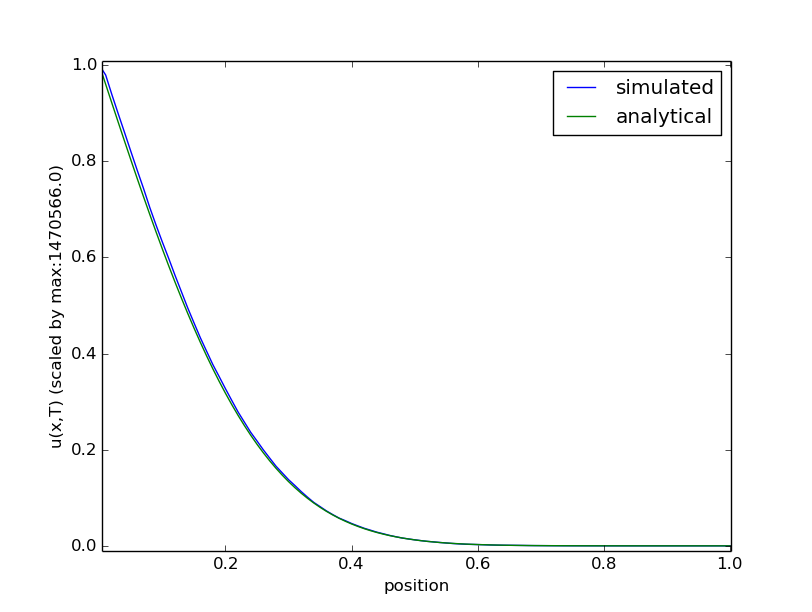
\includegraphics[width=\textwidth]{1DrandomWalk_002.png}
            \caption{time=0.02s}
        \end{subfigure}
        \begin{subfigure}[b!]{0.55\textwidth}
            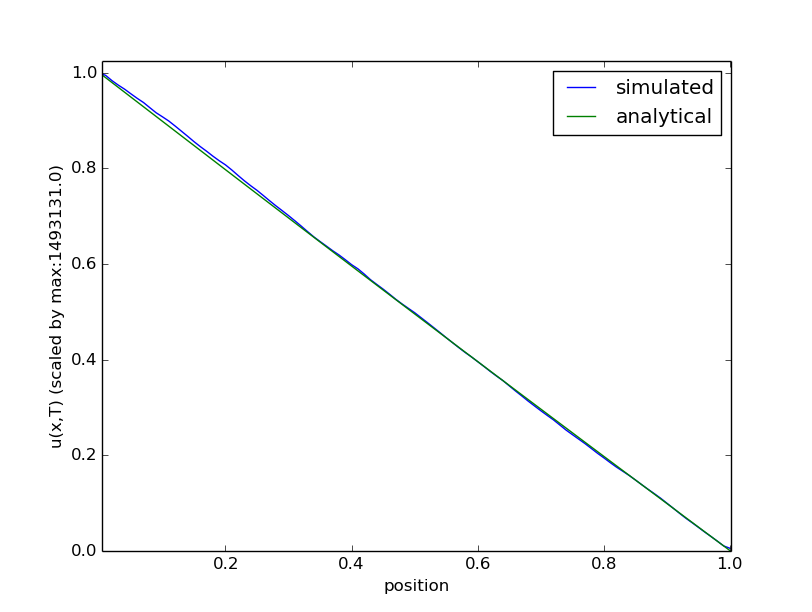
\includegraphics[width=\textwidth]{1DrandomWalk_05.png}
            \caption{time=0.5s}
        \end{subfigure}
    \end{figure}
    \begin{figure}[H]
        \caption{Random walk model $10^3$ walkers $\Delta t = 0.00005$}
        \captionsetup[subfigure]{labelformat=empty}
        \begin{subfigure}[b!]{0.55\textwidth}
            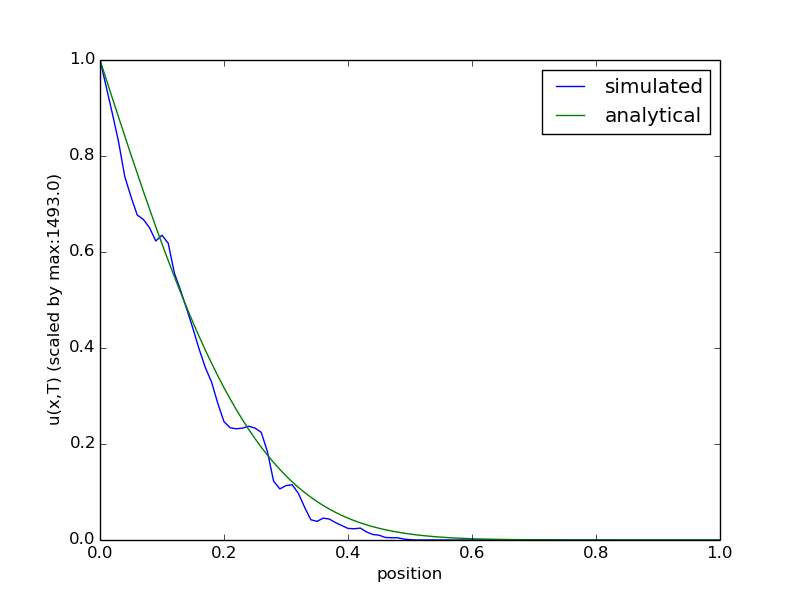
\includegraphics[width=\textwidth]{1DLessRandomWalk_002.png}
            \caption{time=0.02s}
        \end{subfigure}
        \begin{subfigure}[b!]{0.55\textwidth}
            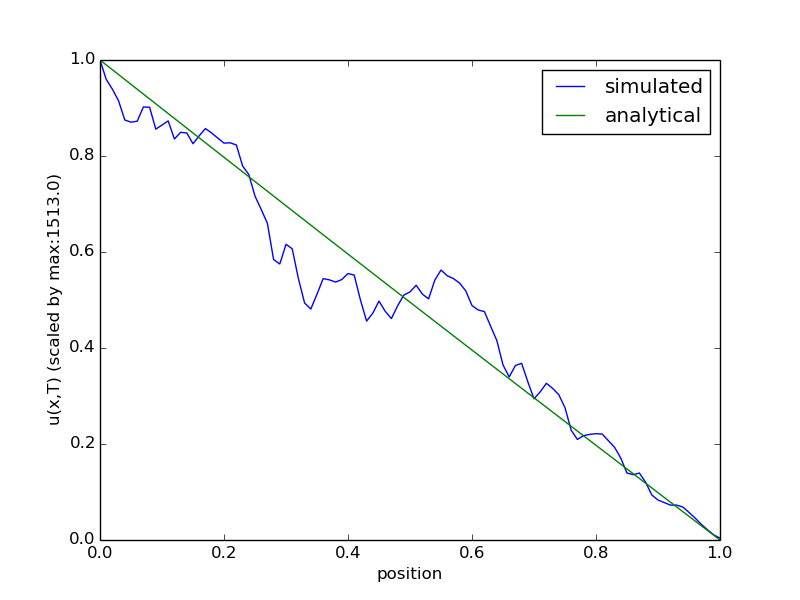
\includegraphics[width=\textwidth]{1DLessRandomWalk_05.png}
            \caption{time=0.5s}
        \end{subfigure}
    \end{figure}

    We can see here that the random walk model is fairly good as long as we keep the number of walkers high. In figure 2 one can see that reducing the number of walkers down to 1000 makes the model somewhat unstable. Also note that the distribution($u(x,T)$) is scaled by its original maximum value. This is done to get a cleaner graph that starts at 1. At $T=0.5$ we observe that the solution is close to the steady state solution.\vsp \\
    As mentioned there was also a model involving a gaussian distribution. The results of those simulations are as follow:
    \begin{figure}[H]
        \caption{Gaussian random walk model $10^6$ walkers $\Delta t = 0.00005$}
        \captionsetup[subfigure]{labelformat=empty}
        \begin{subfigure}[b!]{0.55\textwidth}
            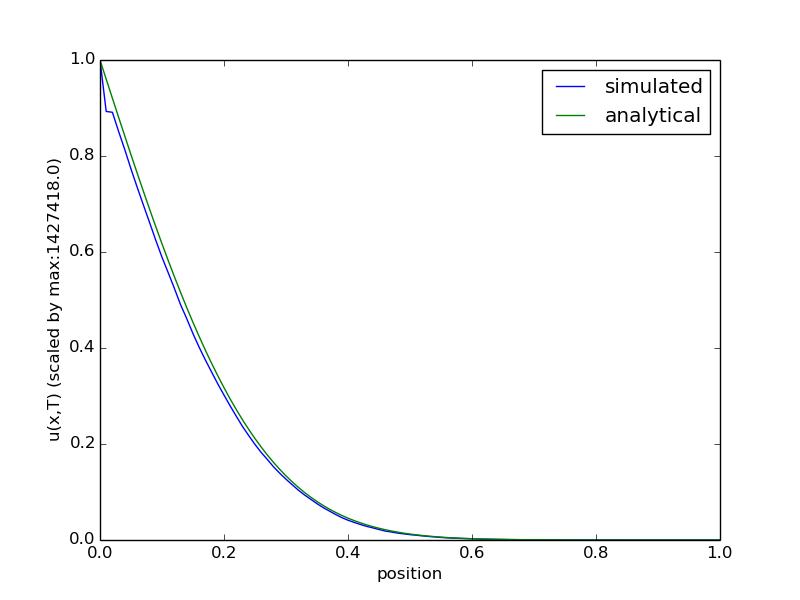
\includegraphics[width=\textwidth]{1Dgauss_002.png}
            \caption{time=0.02s}
        \end{subfigure}
        \begin{subfigure}[b!]{0.55\textwidth}
            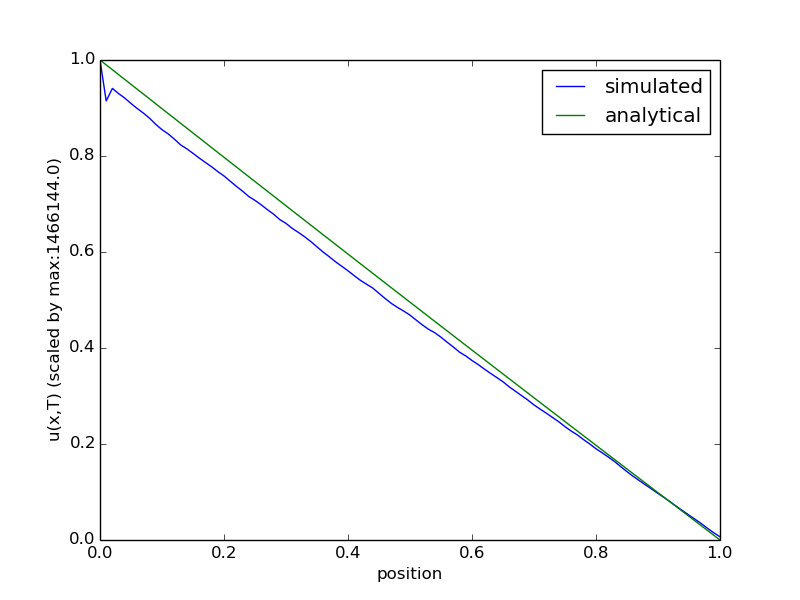
\includegraphics[width=\textwidth]{1Dgauss_05.png}
            \caption{time=0.5s}
        \end{subfigure}
    \end{figure}
    \begin{figure}[H]
        \caption{Gaussian random walk model $10^3$ walkers $\Delta t = 0.00005$}
        \captionsetup[subfigure]{labelformat=empty}
        \begin{subfigure}[b!]{0.55\textwidth}
            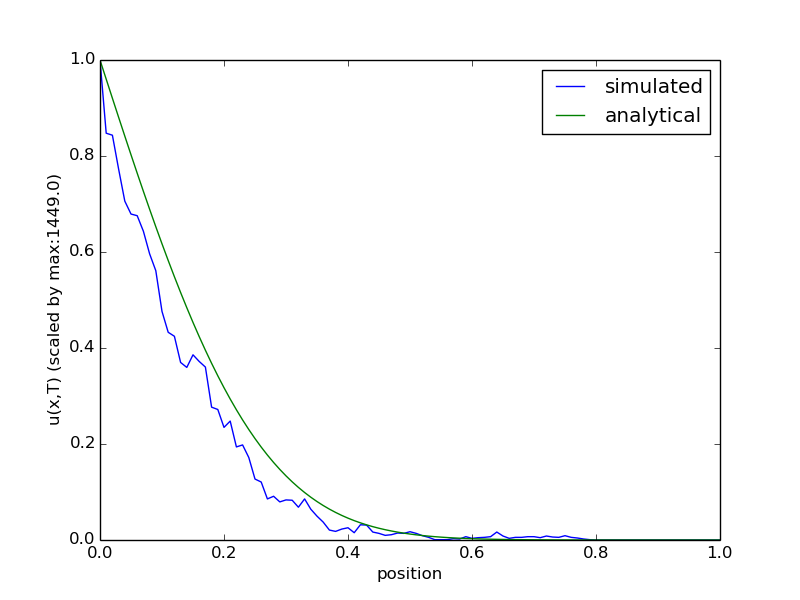
\includegraphics[width=\textwidth]{1DgaussL_002.png}
            \caption{time=0.02s}
        \end{subfigure}
        \begin{subfigure}[b!]{0.55\textwidth}
            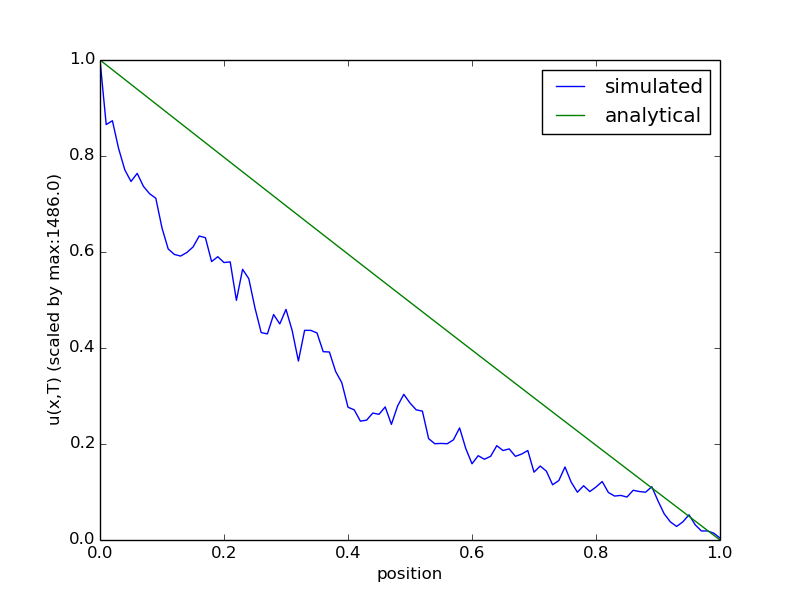
\includegraphics[width=\textwidth]{1DgaussL_05.png}
            \caption{time=0.5s}
        \end{subfigure}
    \end{figure} \justify
    
    The gaussian model seems to actually be worse than the original random walk model, the graphs do not align them selves with the analytical solution as good as previously and reducing the number of walkers obviously made the model worse.\vsp \\
    In the previous project(project 4) we were tasked with implementing an explicit scheme for solving the diffusion equation numerically. The resulting plots were:
    \begin{figure}[H]
        \caption{Explicit forward Euler $\Delta x=1./100, \Delta t=(\Delta x^2/2)$}
        \captionsetup[subfigure]{labelformat=empty}
        \begin{subfigure}[b!]{0.55\textwidth}
            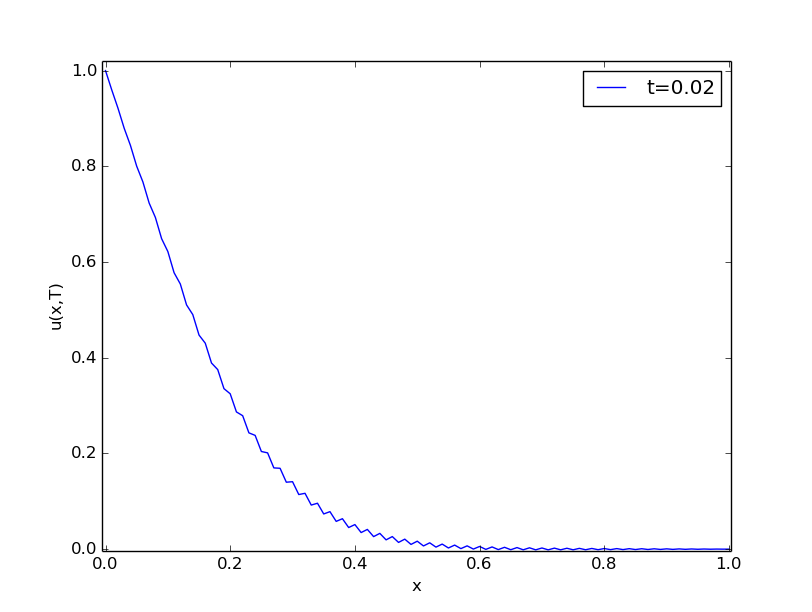
\includegraphics[width=\textwidth]{explicitEuler_002.png}
            \caption{time=0.02s}
        \end{subfigure}
        \begin{subfigure}[b!]{0.55\textwidth}
            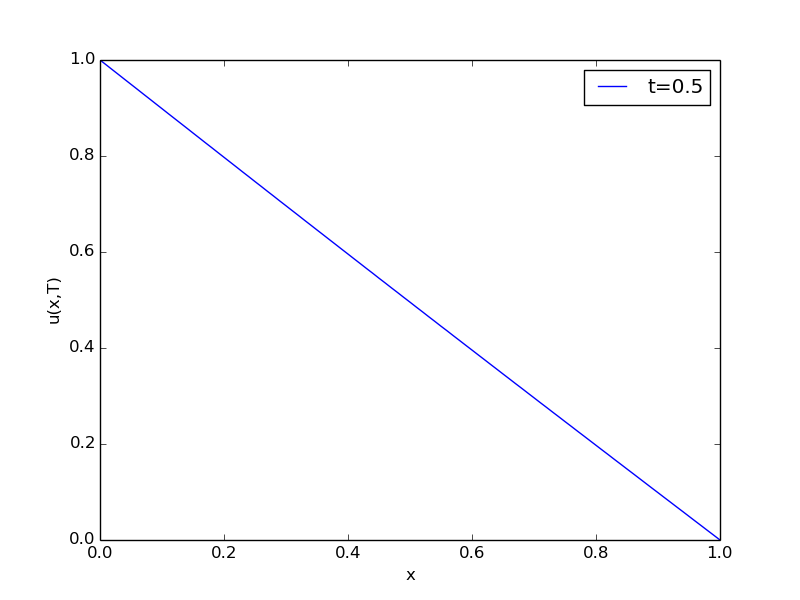
\includegraphics[width=\textwidth]{explicitEuler_05.png}
            \caption{time=0.5s}
        \end{subfigure}
    \end{figure} \justify
    
    The explicit method gets a bit unstable(the graph wobbles) for small time intervals, but is very stable as the time increases and matches very well the steady state solution for $T=0.5$. The unstability comes from the poor stability condition given by:
    
    \begin{equation*}
        \alpha = \frac{\Delta t}{\Delta x^2} \leq \frac{1}{2}
    \end{equation*} \justify
    
    Observe that even with the poor stability condition the solution still seems to be better than the random walk model with the gaussian distribution.

\subsection{Random walk model in two dimensions}
    The plots below are all a gradient plot of x versus y. The colorbar on the side indicates the concentration value(a representation of the function u given by the diffusian equation) and is scaled by the original maximum value.
    \begin{figure}[H]
        \caption{Randomwalk two dimensions $10^6$ walkers $\Delta t=0.000005$}
        \captionsetup[subfigure]{labelformat=empty}
        \begin{subfigure}[b!]{0.55\textwidth}
            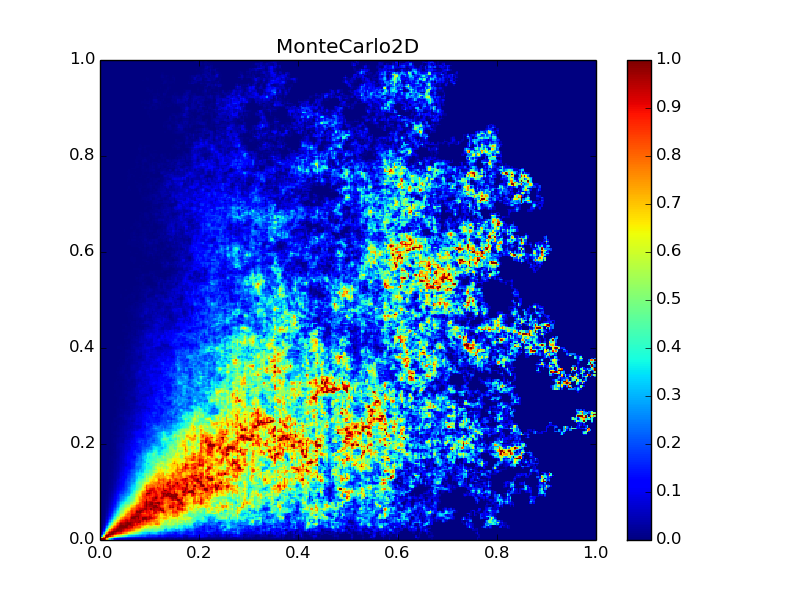
\includegraphics[width=\textwidth]{MC2D_02.png}
            \caption{time=0.2s}
        \end{subfigure}
        \begin{subfigure}[b!]{0.55\textwidth}
            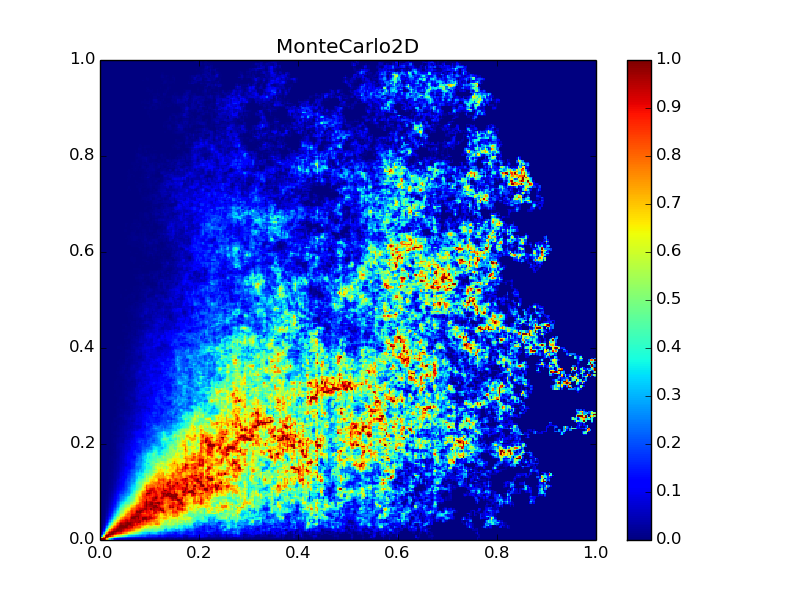
\includegraphics[width=\textwidth]{MC2D_05_2.png}
            \caption{time=0.5s}
        \end{subfigure}
    \end{figure}
    \begin{figure}[H]
        \caption{Randomwalk two dimensions $10^6$ walkers $\Delta t=0.000005$}
        \captionsetup[subfigure]{labelformat=empty}
        \begin{subfigure}[b!]{0.55\textwidth}
            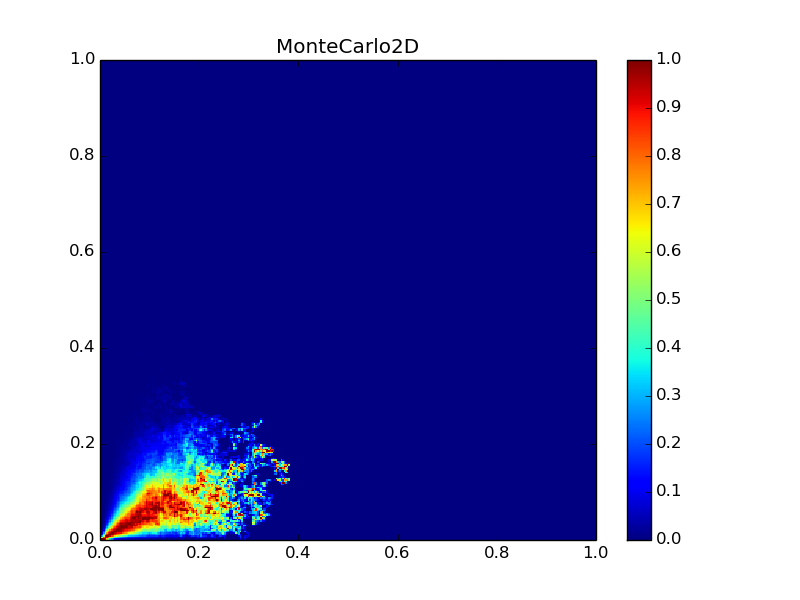
\includegraphics[width=\textwidth]{MC2D_001.png}
            \caption{time=0.01s}
        \end{subfigure}
        \begin{subfigure}[b!]{0.55\textwidth}
            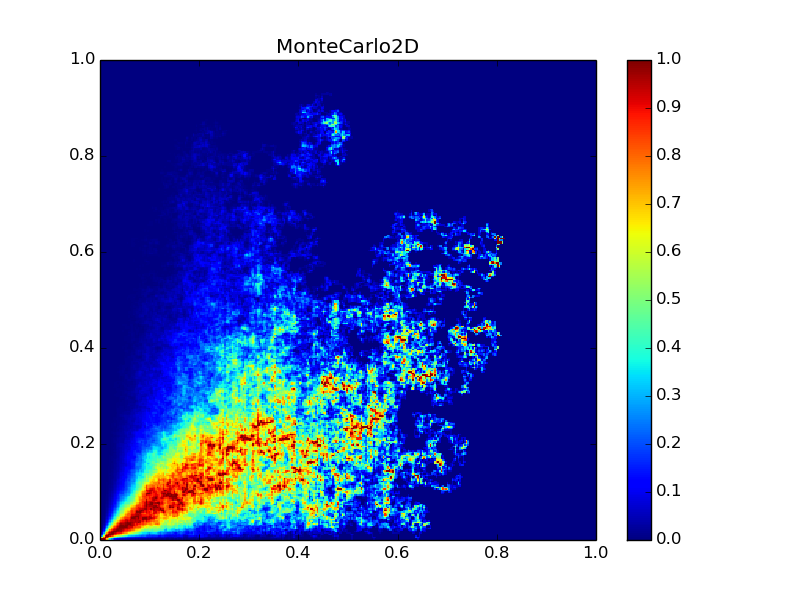
\includegraphics[width=\textwidth]{MC2D_008.png}
            \caption{time=0.08s}
        \end{subfigure}
    \end{figure}
    \begin{figure}[H]
        \caption{Randomwalk two dimensions $10^4$ walkers $\Delta t=0.000005$}
        \captionsetup[subfigure]{labelformat=empty}
        \begin{subfigure}[b!]{0.55\textwidth}
            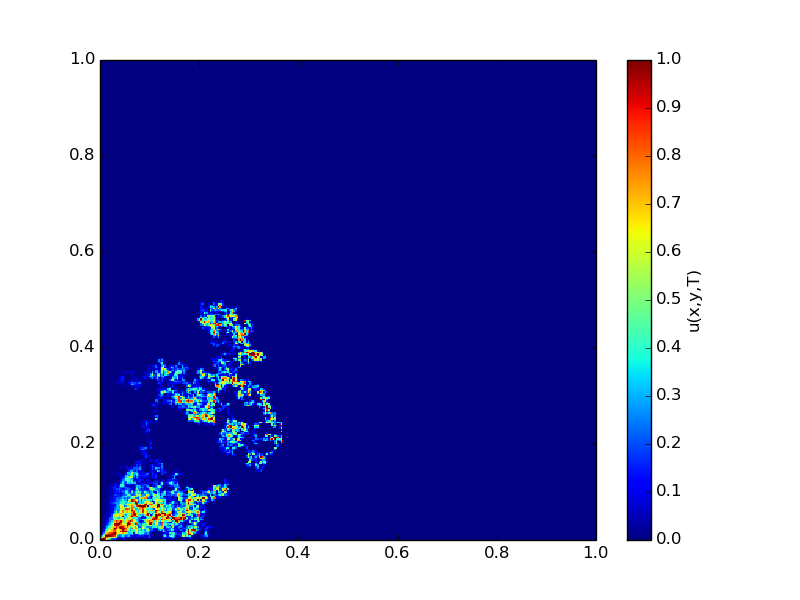
\includegraphics[width=\textwidth]{lMC2D_02.png}
            \caption{time=0.2s}
        \end{subfigure}
        \begin{subfigure}[b!]{0.55\textwidth}
            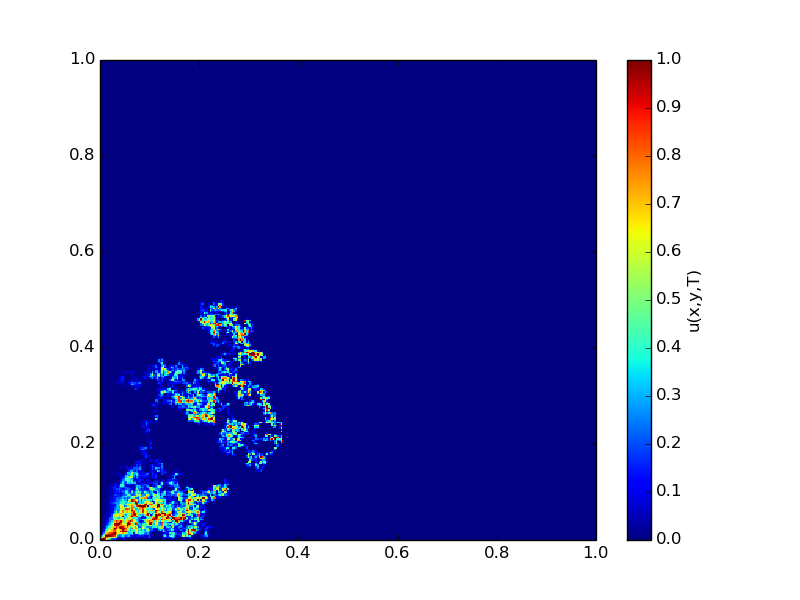
\includegraphics[width=\textwidth]{lMC2D_05.png}
            \caption{time=0.5s}
        \end{subfigure}
    \end{figure}
    \begin{figure}[H]
        \caption{Randomwalk two dimensions $10^6$ walkers $\Delta t=0.0005$}
        \captionsetup[subfigure]{labelformat=empty}
        \begin{subfigure}[b!]{0.55\textwidth}
            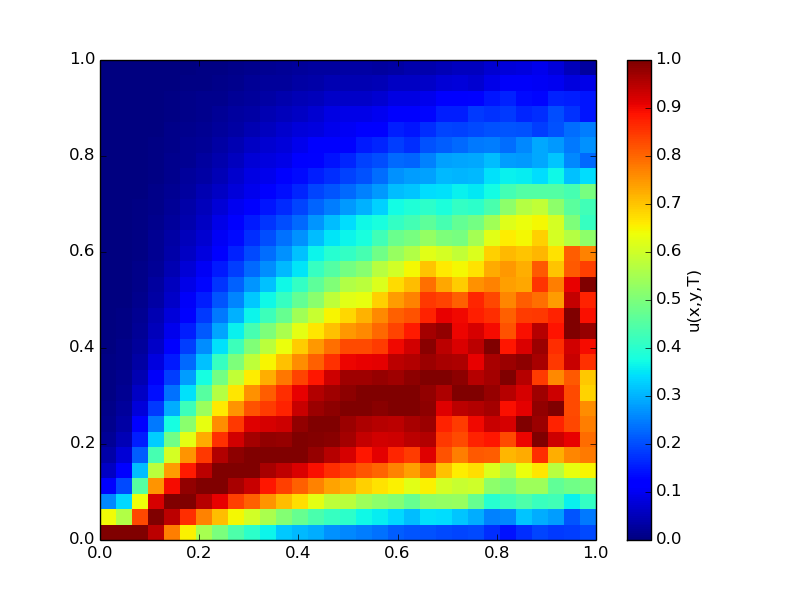
\includegraphics[width=\textwidth]{lMC2Dl_02.png}
            \caption{time=0.2s}
        \end{subfigure}
        \begin{subfigure}[b!]{0.55\textwidth}
            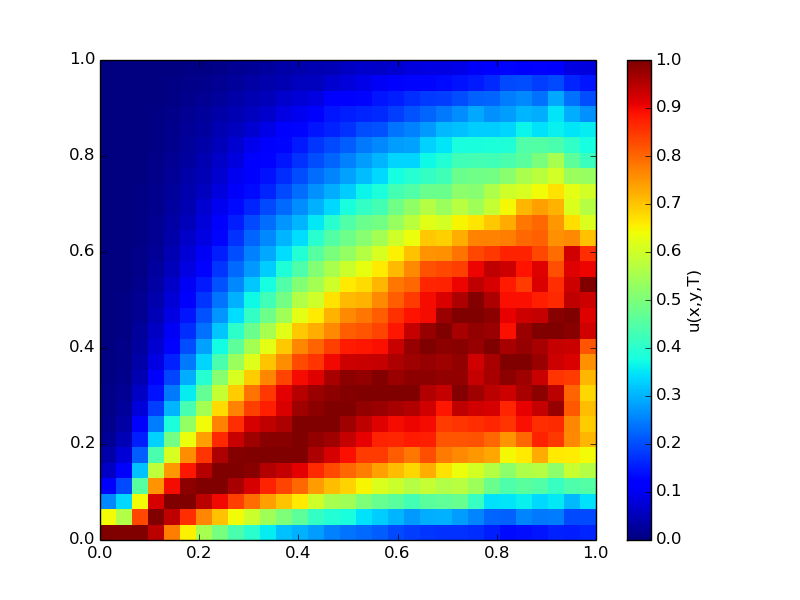
\includegraphics[width=\textwidth]{lMC2Dl_05.png}
            \caption{time=0.5s}
        \end{subfigure}
    \end{figure} \justify

    The resulting plots are looking good and seem to represent a physically natural process of diffusion. It is a natural result that releasing particles in a solvent will make them spread like we see above.\\
    Reducing the number of walker(while maintaining a low time-step) made the plots <<less complete>>. Essentially this just means that there were not enough walkers initially to make a good distribution for the simulation resulting in a poor representation of the diffusion process.\\
    In addition, reducing the time-step offered a pixelated and unclear plot.

\subsection{Analytic solution}
    For the analytic solution we have an actual function that describes the process of diffusion at every meshpoint. The resulting plots incorporate a better flow to them which is good for comparing with the explicit and implicit schemes described above, but for the random walk model the analytical solution is not an accurate base for comparison. The reason for this is described above in section 3.2. The resulting plots:
    \begin{figure}[H]
        \caption{Analytical two dimensions}
        \captionsetup[subfigure]{labelformat=empty}
        \begin{subfigure}[b!]{0.55\textwidth}
            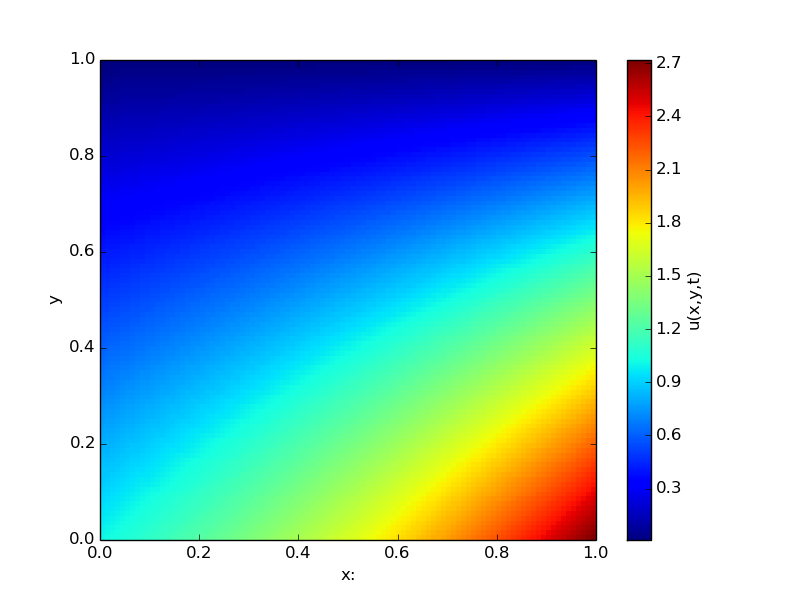
\includegraphics[width=\textwidth]{analytic2D_001.png}
            \caption{time=0.01s}
        \end{subfigure}
        \begin{subfigure}[b!]{0.55\textwidth}
            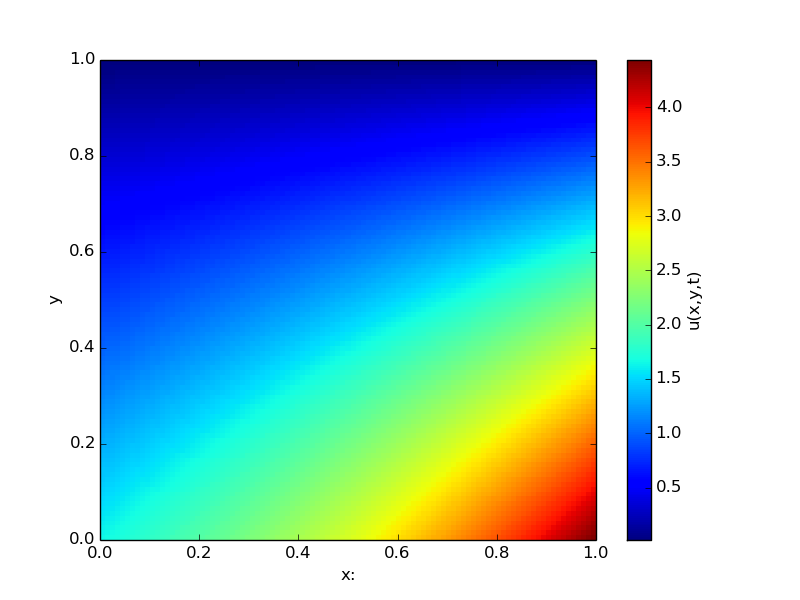
\includegraphics[width=\textwidth]{analytic2D_05.png}
            \caption{time=0.5s}
        \end{subfigure}
    \end{figure}
    
    As presumed the plots have a better flow to them, the solutions at different time-values look pretty much exactly the same, but the concentration is much larger as the time increses(see the colorbars). The concentration is here initiated at 1 since $u(0,0,0)=1$.

\subsection{Explicit scheme}
    Here we will plot the explicit scheme with the stability criteria sustained and also when it is not.
    \begin{figure}[H]
        \caption{Explicit scheme $\Delta t=0.000005$}
        \captionsetup[subfigure]{labelformat=empty}
        \begin{subfigure}[b!]{0.55\textwidth}
            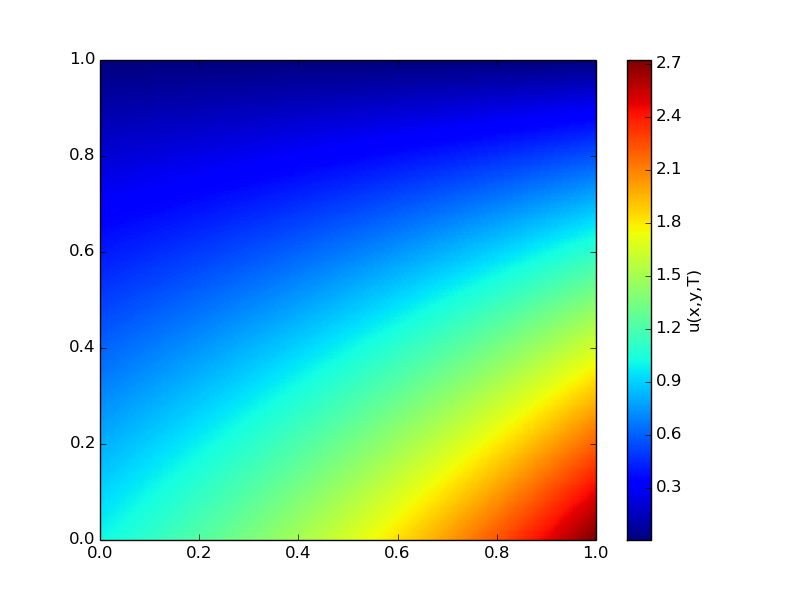
\includegraphics[width=\textwidth]{explicit2D_001.png}
            \caption{time=0.01s}
        \end{subfigure}
        \begin{subfigure}[b!]{0.55\textwidth}
            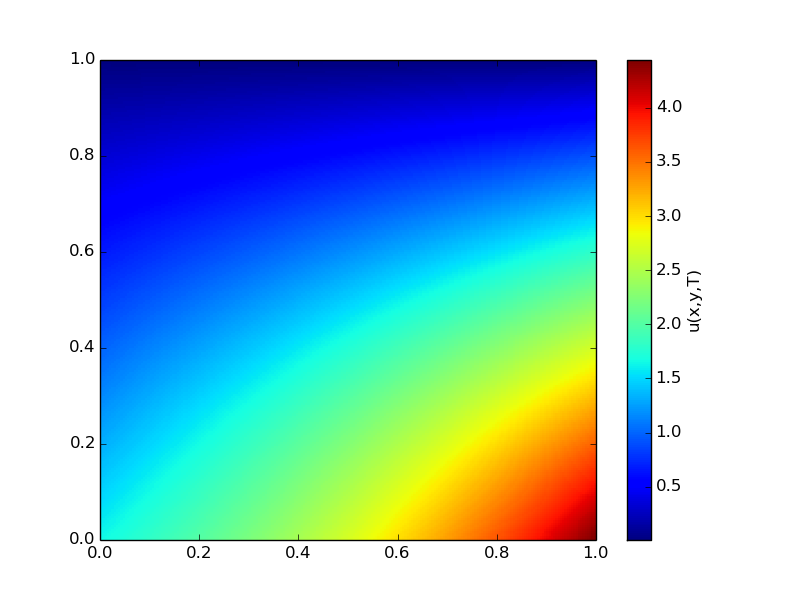
\includegraphics[width=\textwidth]{explicit2D_05.png}
            \caption{time=0.5s}
        \end{subfigure}
    \end{figure}
    \begin{figure}[H]
        \caption{Explicit scheme $\Delta t=0.005$}
        \captionsetup[subfigure]{labelformat=empty}
        \begin{subfigure}[b!]{0.55\textwidth}
            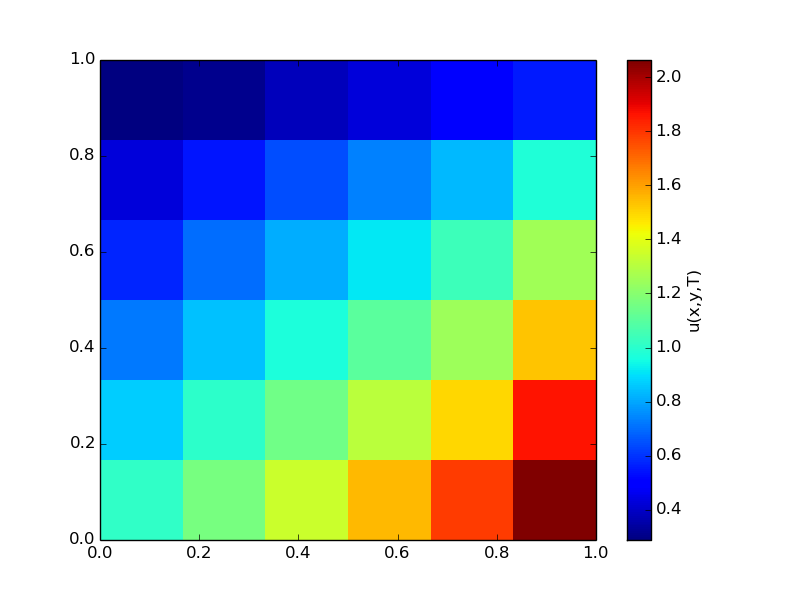
\includegraphics[width=\textwidth]{lExplicit2D_001.png}
            \caption{time=0.01s}
        \end{subfigure}
        \begin{subfigure}[b!]{0.55\textwidth}
            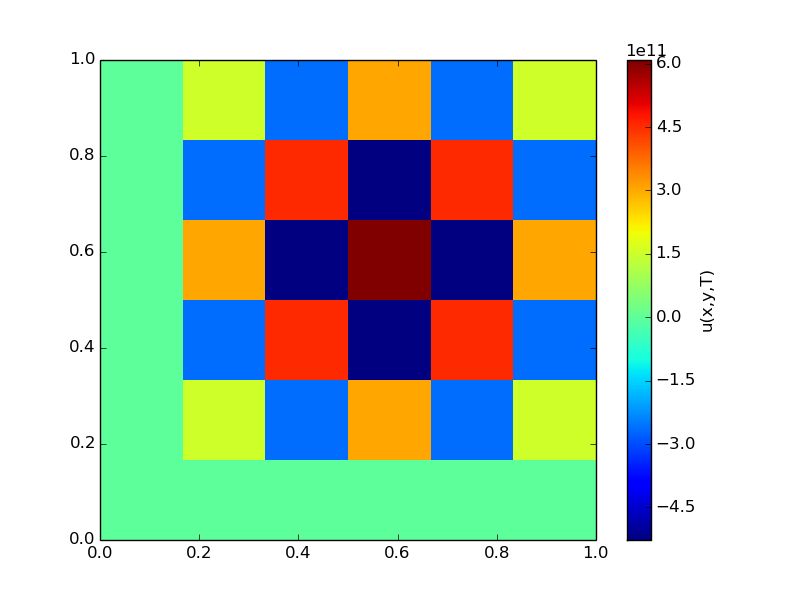
\includegraphics[width=\textwidth]{lExplicit2D_05.png}
            \caption{time=0.5s}
        \end{subfigure}
    \end{figure}
    \begin{figure}[H]
        \caption{Explicit scheme unstable}
        \centering
        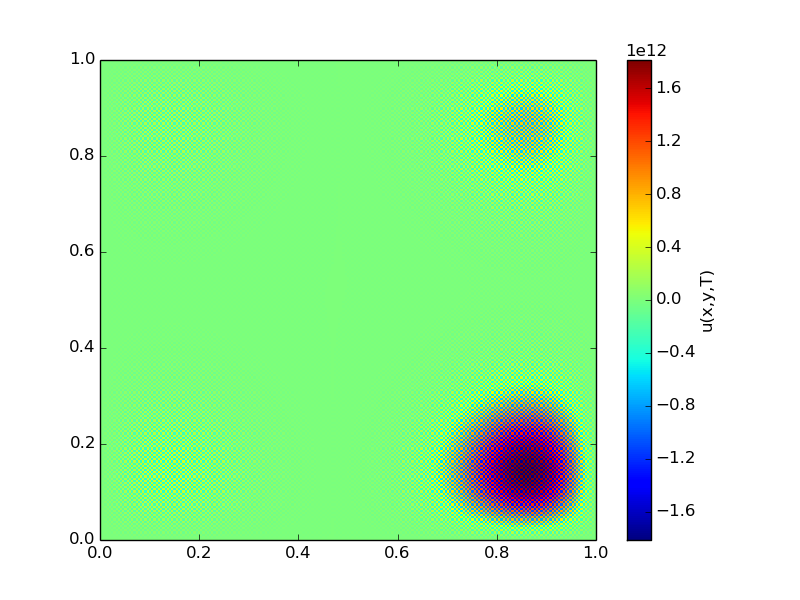
\includegraphics[scale=0.5]{explicit2D_unstable.png}
    \end{figure}
    
    As long as the stability criteria is sustained the explicit scheme works well for low values of $\Delta t$, but the moment the stability criteria is not upheld the solution gets ridiculously unstable. 

\newpage

\subsection{Implicit scheme}
    The implicit scheme will always be stable for any combination of $\Delta t$ and $\Delta x$. The results look like these.
    
    \begin{figure}[H]
        \caption{Implicit scheme $\Delta t=0.00005$}
        \captionsetup[subfigure]{labelformat=empty}
        \begin{subfigure}[b!]{0.55\textwidth}
            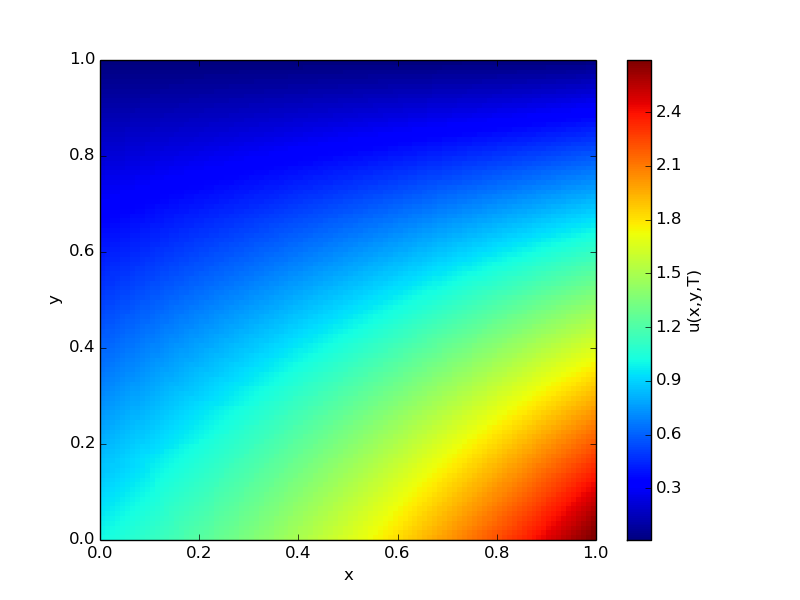
\includegraphics[width=\textwidth]{implicit2D_001.png}
            \caption{time=0.01s}
        \end{subfigure}
        \begin{subfigure}[b!]{0.55\textwidth}
            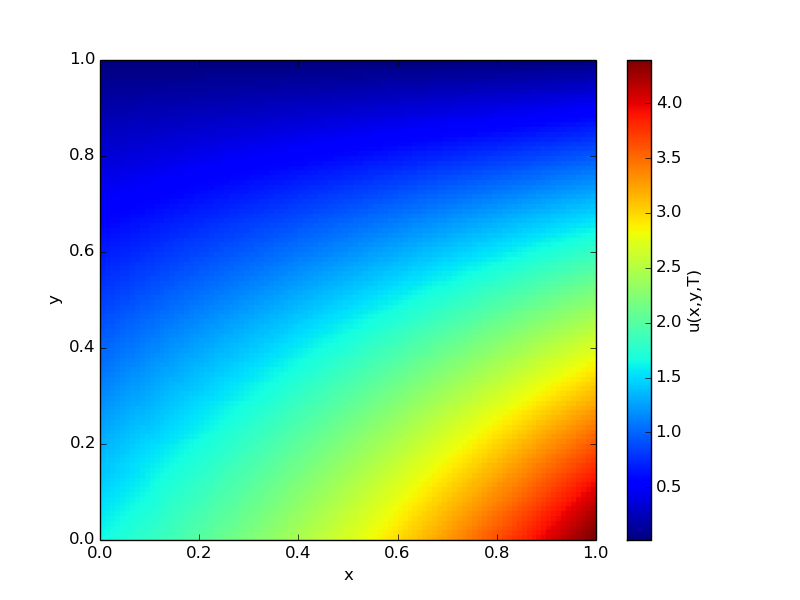
\includegraphics[width=\textwidth]{implicit2D_05.png}
            \caption{time=0.5s}
        \end{subfigure}
    \end{figure}
    \begin{figure}[h]
        \caption{Implicit scheme $\Delta t=0.005$}
        \captionsetup[subfigure]{labelformat=empty}
        \begin{subfigure}[b!]{0.55\textwidth}
            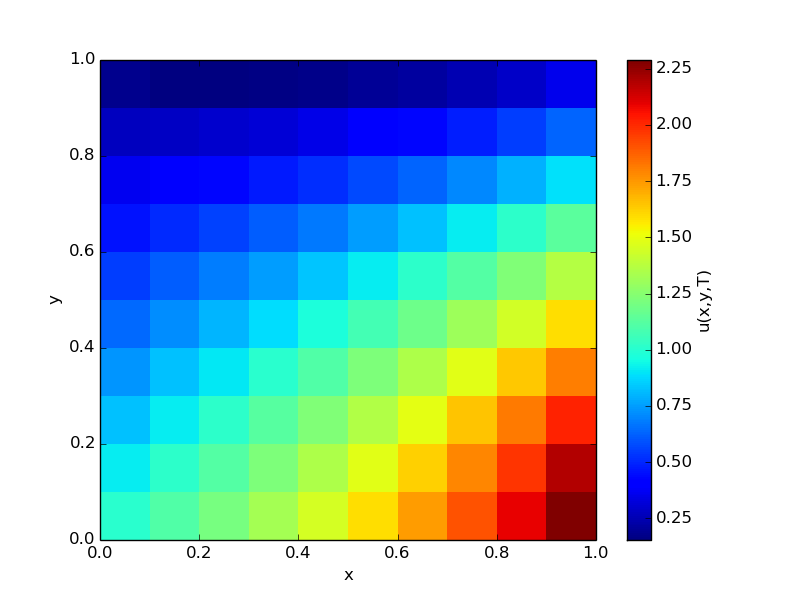
\includegraphics[width=\textwidth]{limplicit2D_001.png}
            \caption{time=0.01s}
        \end{subfigure}
        \begin{subfigure}[b!]{0.55\textwidth}
            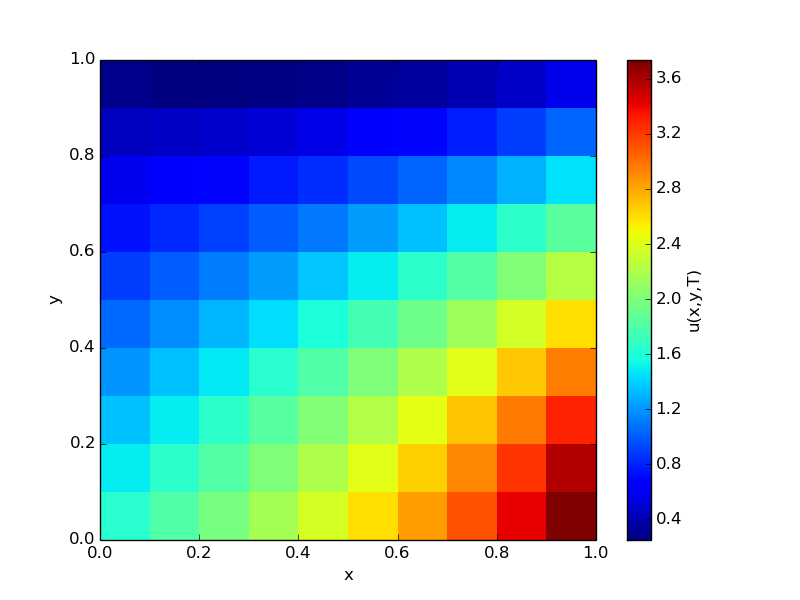
\includegraphics[width=\textwidth]{limplicit2D_05.png}
            \caption{time=0.5s}
        \end{subfigure}
    \end{figure}
    
    As we can see the implicit scheme is still very much stable.

\secti{Error estimates}
    This section will cover error estimates for the different methods and schemes used in the sections above.

\subsection{Error random walk 1D }
    \begin{figure}[H]
        \caption{Error random walk model $10^6$ walkers $\Delta t=0.00005$}
        \captionsetup[subfigure]{labelformat=empty}
        \begin{subfigure}[b!]{0.55\textwidth}
            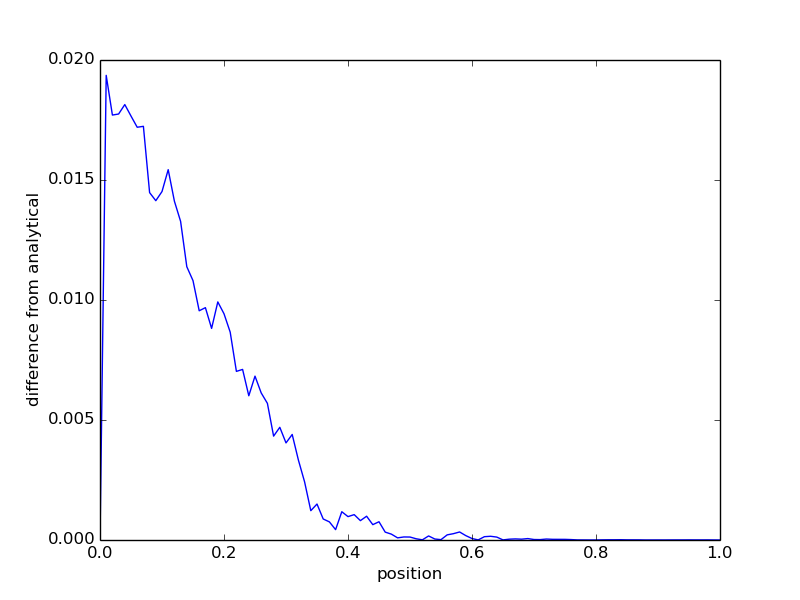
\includegraphics[width=\textwidth]{randomWalk1D_error_002.png}
            \caption{time=0.02s}
        \end{subfigure}
        \begin{subfigure}[b!]{0.55\textwidth}
            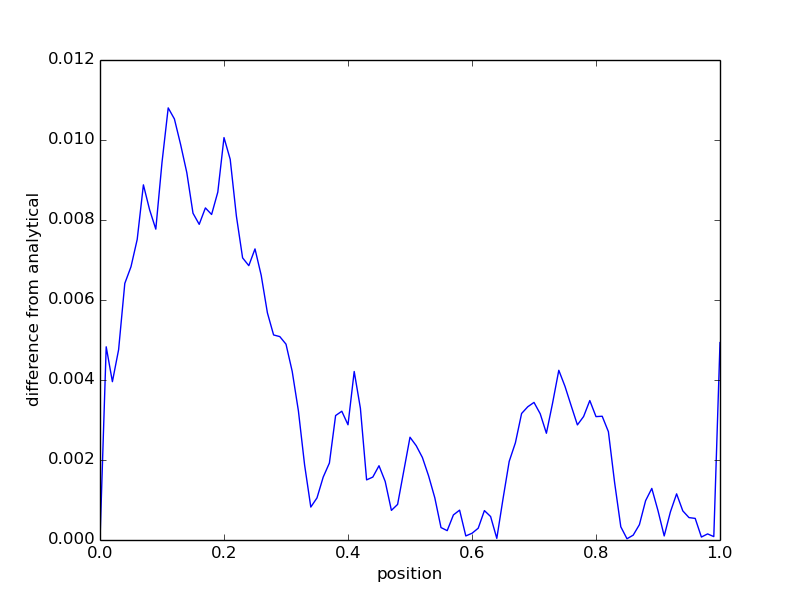
\includegraphics[width=\textwidth]{randomWalk1D_error_05.png}
            \caption{time=0.5s}
        \end{subfigure}
    \end{figure}
    \begin{figure}[H]
        \caption{Error random walk model $10^4$ walkers $\Delta t=0.0005$}
        \captionsetup[subfigure]{labelformat=empty}
        \begin{subfigure}[b!]{0.55\textwidth}
            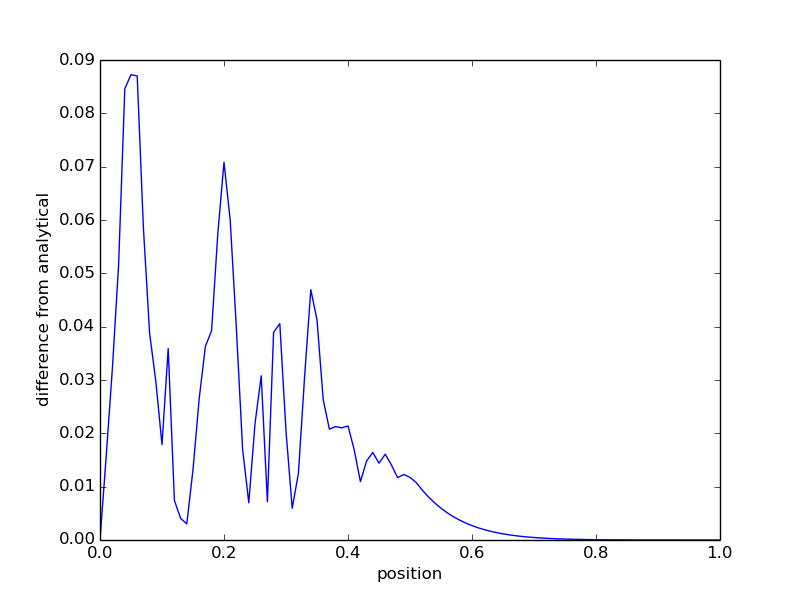
\includegraphics[width=\textwidth]{lrandomWalk1D_error_002.png}
            \caption{time=0.02s}
        \end{subfigure}
        \begin{subfigure}[b!]{0.55\textwidth}
            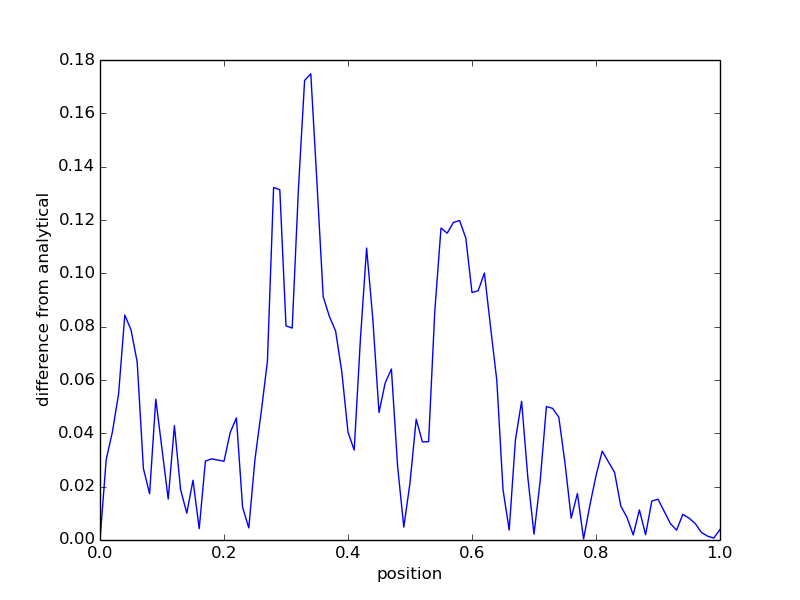
\includegraphics[width=\textwidth]{lrandomWalk1D_error_05.png}
            \caption{time=0.5s}
        \end{subfigure}
    \end{figure}
    
    Here we observe that the error is considerably low if we have a large number of walkers, however the error increses as the total time increases. When the number of walkers is reduced the error gets very much present and we can see that for $T=0.5$ the maximum spike is up at 0.17 which is quite large.

\subsection{Error random walk 1D with gauss}
    \begin{figure}[H]
        \caption{Error random walk gauss $10^6$ walkers $\Delta t=0.00005$}
        \captionsetup[subfigure]{labelformat=empty}
        \begin{subfigure}[b!]{0.55\textwidth}
            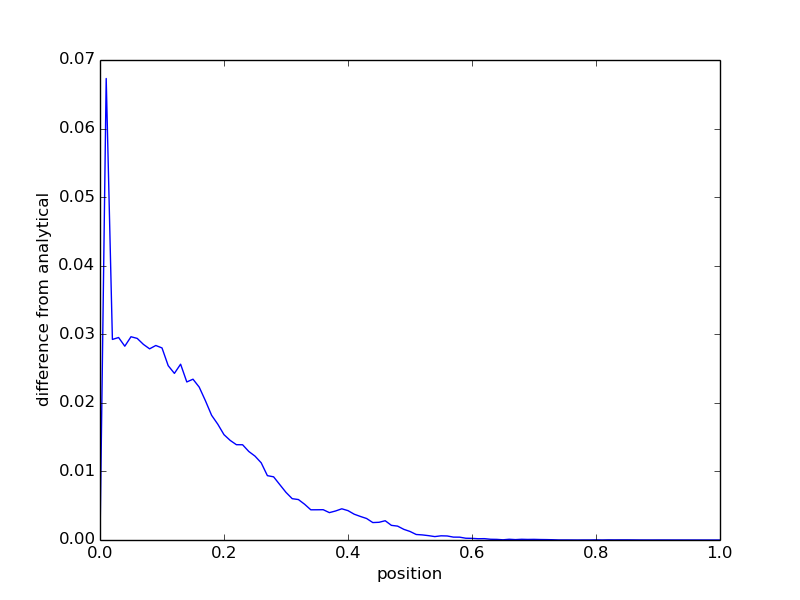
\includegraphics[width=\textwidth]{randomWalkGauss1D_error_002.png}
            \caption{time=0.02s}
        \end{subfigure}
        \begin{subfigure}[b!]{0.55\textwidth}
            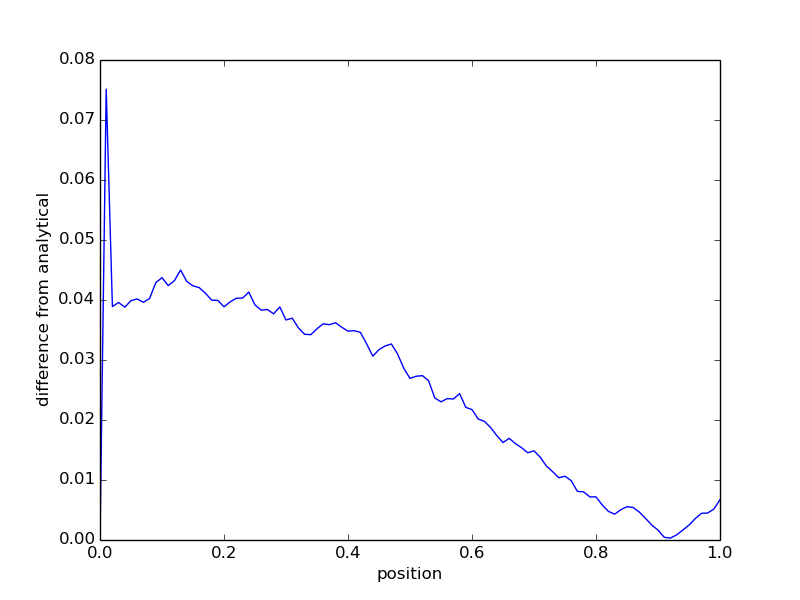
\includegraphics[width=\textwidth]{randomWalkGauss1D_error_05.png}
            \caption{time=0.5s}
        \end{subfigure}
    \end{figure}
    \begin{figure}[H]
        \caption{Error random walk gauss $10^4$ walkers $\Delta t=0.0005$}
        \captionsetup[subfigure]{labelformat=empty}
        \begin{subfigure}[b!]{0.55\textwidth}
            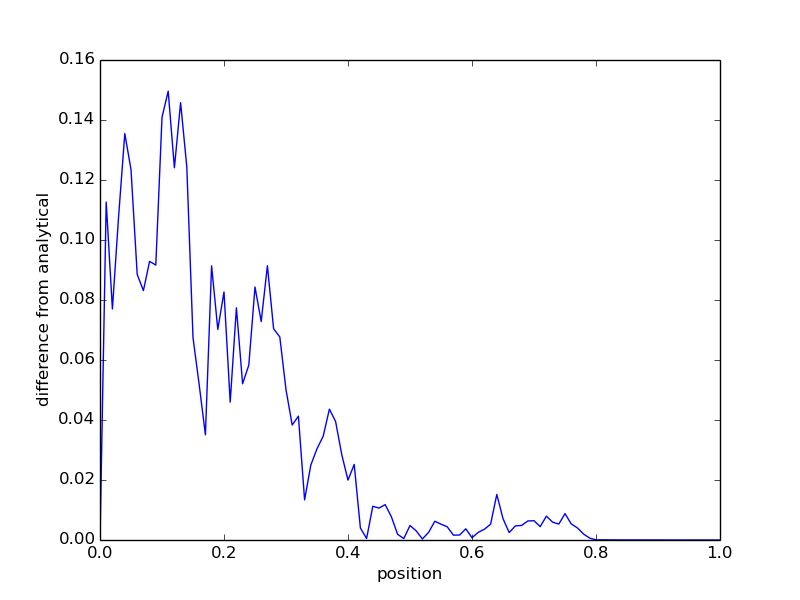
\includegraphics[width=\textwidth]{lrandomWalkGauss1D_error_002.png}
            \caption{time=0.02s}
        \end{subfigure}
        \begin{subfigure}[b!]{0.55\textwidth}
            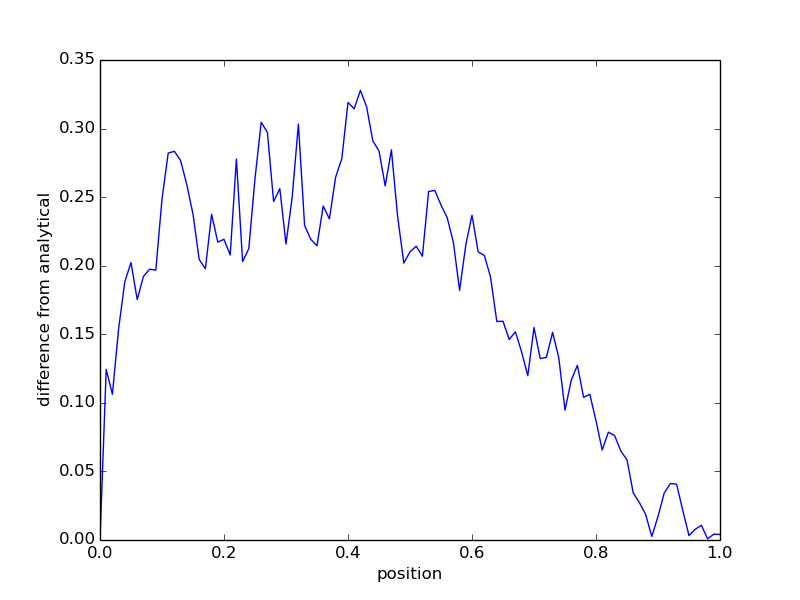
\includegraphics[width=\textwidth]{lrandomWalkGauss1D_error_05.png}
            \caption{time=0.5s}
        \end{subfigure}
    \end{figure} \justify

    With the extra gaussian distribution the model actually gets worse. The error has a big spike in the beginning before decreasing, however the decrease is much slower than before and the overall error is still larger. An increased total time also increased the error here aswell. The natural presumption for the results with the gaussian model is that it should be better, we are introducing a distribution which should give more values around the desired criteria which in turn should give a better result. Also reducing the number of walkers obviously did not yield any better results.
\subsection{Error explicit scheme}
    \begin{figure}[H]
        \caption{Error explicit scheme $\Delta t=0.00005$}
        \captionsetup[subfigure]{labelformat=empty}
        \begin{subfigure}[b!]{0.55\textwidth}
            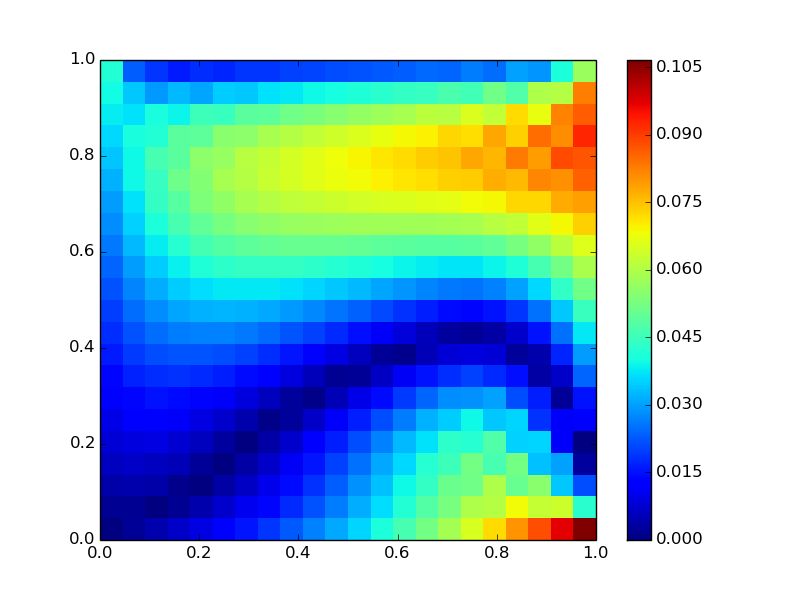
\includegraphics[width=\textwidth]{explicit2D_error_001.png}
            \caption{time=0.01s}
        \end{subfigure}
        \begin{subfigure}[b!]{0.55\textwidth}
            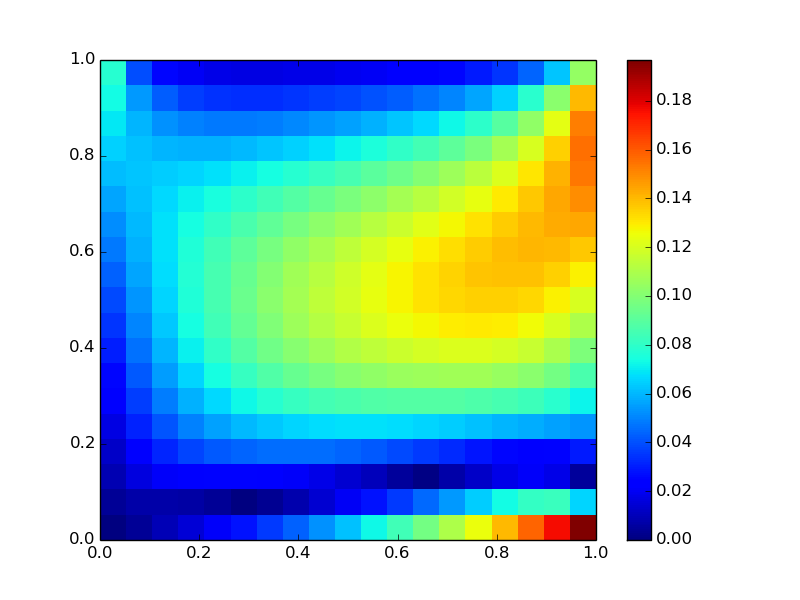
\includegraphics[width=\textwidth]{explicit2D_error_05.png}
            \caption{time=0.5s}
        \end{subfigure}
    \end{figure}
    
    For the explicit scheme the error estimates are also done by checking the difference from the analytical solution. We can see that the error is large at the initial position but overall actually fairly good. For $T=0.5$ the error is actually very large.

\subsection{Error implicit scheme}
    \begin{figure}[H]
        \caption{Error implicit scheme $\Delta t=0.00005$}
        \captionsetup[subfigure]{labelformat=empty}
        \begin{subfigure}[b!]{0.55\textwidth}
            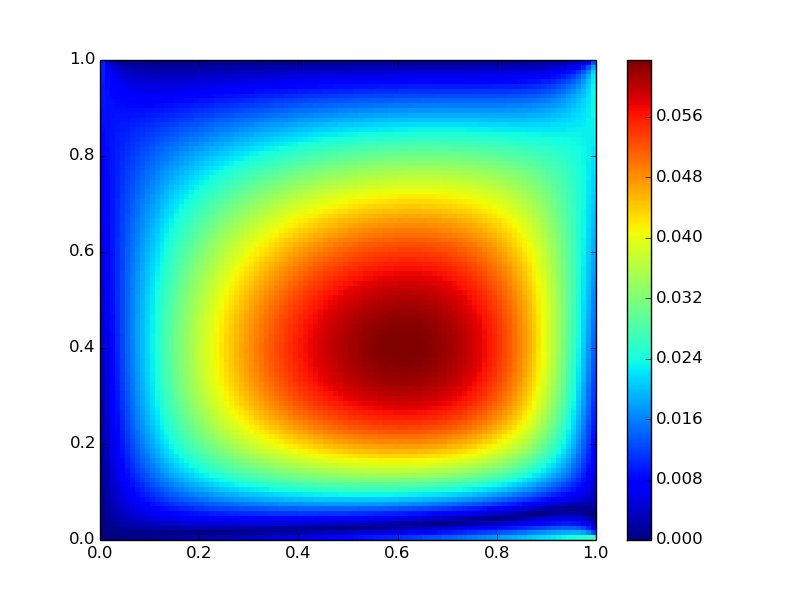
\includegraphics[width=\textwidth]{implicit2D_error_001.png}
            \caption{time=0.01s}
        \end{subfigure}
        \begin{subfigure}[b!]{0.55\textwidth}
            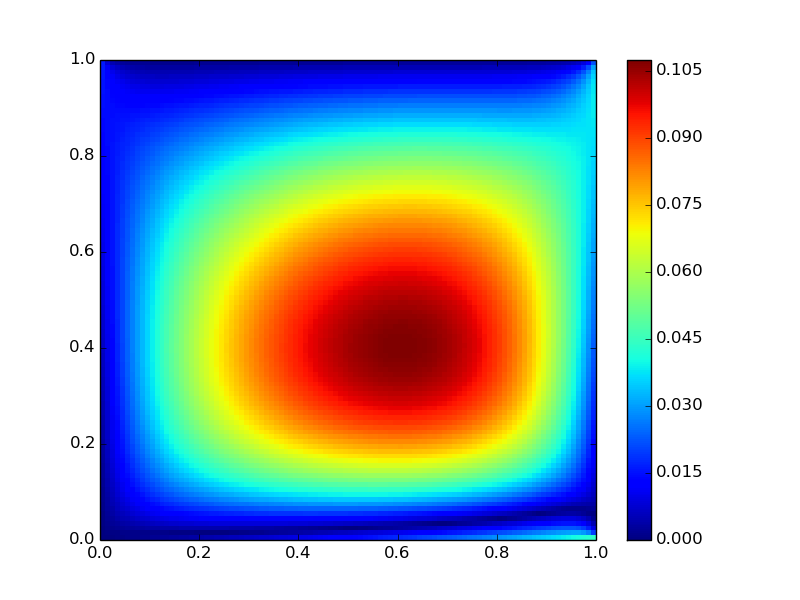
\includegraphics[width=\textwidth]{implicit2D_error_05.png}
            \caption{time=0.5s}
        \end{subfigure}
    \end{figure}
    \begin{figure}[H]
        \caption{Error implicit scheme $\Delta t=0.0005$}
        \captionsetup[subfigure]{labelformat=empty}
        \begin{subfigure}[b!]{0.55\textwidth}
            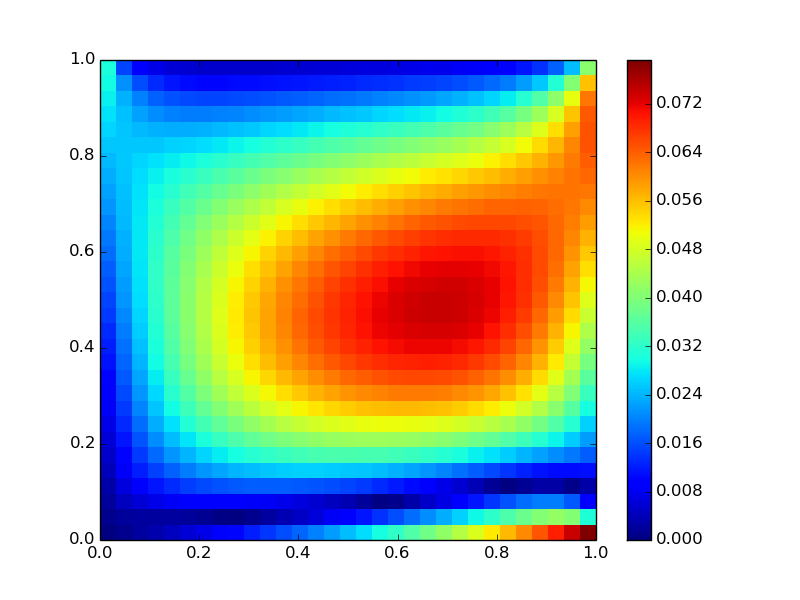
\includegraphics[width=\textwidth]{limplicit2D_error_001.png}
            \caption{time=0.01s}
        \end{subfigure}
        \begin{subfigure}[b!]{0.55\textwidth}
            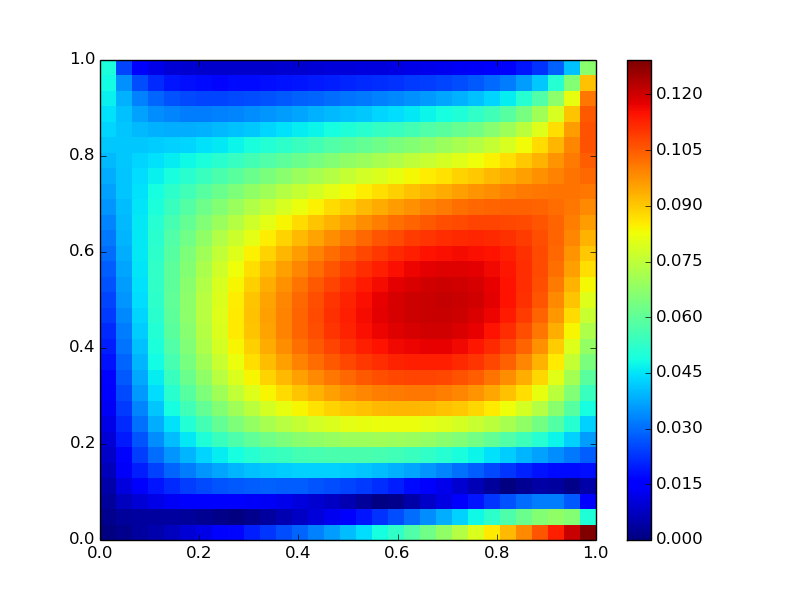
\includegraphics[width=\textwidth]{limplicit2D_error_05.png}
            \caption{time=0.5s}
        \end{subfigure}
    \end{figure} \justify

    The implicit scheme seems to be the favorable one, atleast when we look at the error estimates. The overall error is actually fairly low and the largest peak for $T=0.5$ is 0.11, which is considerably lower than that of the explicit scheme. Note that the peak error stations itself in the middle, while the explicit method has errors everywhere. This behaviour might not be the most favorable for every situation, but atleast one can borderline the error and somewhat confine it. Increasing the time-step naturally gave a larger error.

\secti{Conclusion}
    This section is mainly for conluding the various results that were found in previous sections and to offer some critial views on the project itself.

\subsection{Random walk model}
    The random walk model in 1D actually turned out to be somewhat applicable, however not good enough. Even with a large number of walkers and a low time-step the model couldn't reach the analytical solution very well. It worked considerably good for small time-values, but as the time increased towards the steady-state solution the graphs did not align very well. Besides, reducing the number of walkers also rendered the model mainly useless. On the positive side the model seemed to be fairly stable, altough it jumped around the analytical solution alot, it actually jumped around rather than <<fly off into the sunset>>, that is get unstable and blow up.\vsp \\
    We also observed that the gaussian distribution surprisingly resulted in worse results. The errors very larger, and it was slightly less stable aswell. This result may have many reasons, but the main concern is probably the fact that different seeds were not experimented with. The random number generator was also not the most optimal one giving raise to failure.\vsp \\
    The random walk model was also compared to the explicit scheme(in one dimension). The problem with the explicit scheme from previous project was that it had a poor stability criteria, giving raise to instabilites. The stable plots were also a bit unstable as it <<wobbled>> since the time-step was to high. Still the explicit method was actually better than the random walk model with the gaussian distribution.

\subsection{Random walk in two dimensions}
    In two dimensions the random walk turned out to be very good. The results gave a very intuitive look at the diffusion process. One could see the fluctuations and the concentration levels decrease as the particles moved away from the initial dispersion point.\\
    The model also seemed very stable for all the tested time-values, including close to the steady-state. In addition reducing the number of walkers did not create any instabilites, the only concern was that the process itself was not replicated correctly. There simply weren't enough walkers to represent all the particles so the resulting plot was an <<incomplete>> representation of the diffusion process.\vsp \\
    Reducing the time-step naturally resulted in poor resolution of the plot.\vsp \\
    The error in the implementation was not taken into account in this project because the boundary conditions used for the random walk model did not have any analytical solution. For a more realistic problem this method needs more testing and alot more experimenting in order to keep the stability under check. With that said, the method itself proved to be very stable giving raise to higher probability of promising results. Plus the plots look really cool!

\subsection{Explicit and implicit schemes}
    The explicit scheme with the forward Euler formula actually gave good results, aslong as the stability criteria was under control. The problem with the method was that choosing a larger time-value with a low time-step gave very unstable results and the moment the stability criteria wasn't archieved, the values blew up.\\
    The explicit scheme is very simple to implement, but the poor stability condition deems it useless in most cases. In the situation of the diffusion equation the scheme seems viable, but the implicit method showed itself to be better. Both the error estimates were better for the implicit method compared to the explicit one. The most alarming fact about the explicit scheme was that the error was both large and distributed. The errors for the implicit scheme centered itself while the explicit had some error at the initial point while it decreased as one moved out and then it increased again. Giving raise to some concerns about instabilites.\\
    The implicit scheme on the other hand gave some very good results as mentioned. The error was lower and it was very much stable. The concern about the method is however that it has a slow convergence criteria making it fairly slow scheme, but it too was easy to implement.\\ 
    The essential part about choosing the implicit scheme over the explicit one is obviously the stability criteria, where the explicit scheme has a poor stability condition the implicit one is actually always(sort of) stable. The only problem is that it is actually fairly slow and has a convergence criteria that can be a hassle to handle for some situations. In case of the diffusion equation the convergence threshold proved to be very straight forward to implement.

\newpage
\secti{Sources}
\textbf{Project from 2012}\\
\url{http://www.uio.no/studier/emner/matnat/fys/FYS3150/h12/undervisningsmateriale/projects/project-5\%3A-diffusion-equation/project5\_diffusion2012.pdf}\\
The analytical solution for the two-dimensional equation was taken from here.\vsp \\
\textbf{The project text}\\
\url{http://www.uio.no/studier/emner/matnat/fys/FYS3150/h14/undervisningsmateriale/projects/project-5-deadline-december-1/project5\_diffusion.pdf}\\
Heavily used for the theory part.\vsp \\
\textbf{The lectur notes in computational physics by Morten Hjorth-Jensen}\\
\url{http://www.uio.no/studier/emner/matnat/fys/FYS3150/h14/undervisningsmateriale/Lecture\%20Notes/lecture2014.pdf}
Chapter 10.2 and 10.3 for explicit and implicit scheme along with analytical solution to one-dimensional equation. Chapter 11.3 for randomnumber generator. Chapter 12.2 for random walk model.
\end{document}
